
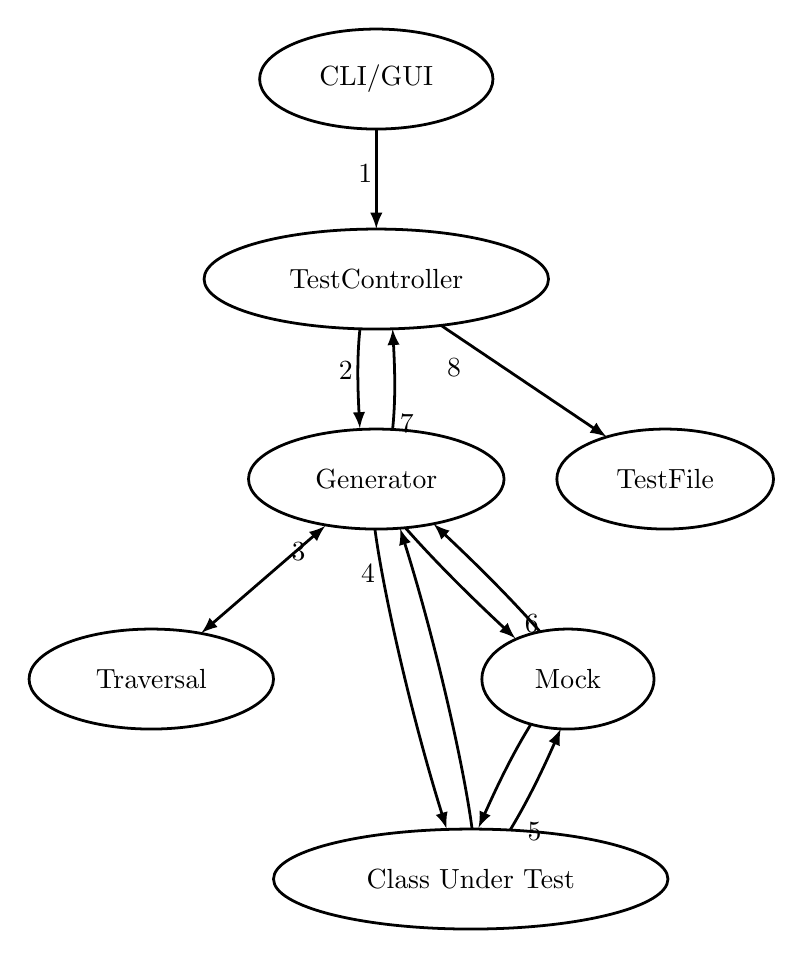
\begin{tikzpicture}[>=latex,line join=bevel,]
  \pgfsetlinewidth{1bp}
%%
\pgfsetcolor{black}
  % Edge: Generator -> TestController
  \draw [->] (130.91bp,180.28bp) .. controls (131.71bp,188.03bp) and (131.94bp,197.36bp)  .. (130.88bp,216.05bp);
  \definecolor{strokecol}{rgb}{0.0,0.0,0.0};
  \pgfsetstrokecolor{strokecol}
  \draw (136bp,182bp) node {7};
  % Edge: TestController -> TestFile
  \draw [->] (148.34bp,217.29bp) .. controls (163.4bp,207.16bp) and (183.12bp,193.88bp)  .. (207.86bp,177.23bp);
  \draw (153bp,202bp) node {8};
  % Edge: Class Under Test -> Mock
  \draw [->] (173.26bp,35.789bp) .. controls (178.15bp,43.848bp) and (183.31bp,53.694bp)  .. (191.41bp,72.055bp);
  \draw (182bp,35bp) node {5};
  % Edge: Mock -> Class Under Test
  \draw [->] (180.51bp,73.465bp) .. controls (175.48bp,65.334bp) and (170.1bp,55.147bp)  .. (161.8bp,36.461bp);
  % Edge: Class Under Test -> Generator
  \draw [->] (159.46bp,36.268bp) .. controls (156.18bp,60.714bp) and (145.69bp,105.63bp)  .. (133.59bp,144.15bp);
  % Edge: CLI/GUI -> TestController
  \draw [->] (125bp,287.7bp) .. controls (125bp,279.98bp) and (125bp,270.71bp)  .. (125bp,252.1bp);
  \draw (121bp,272bp) node {1};
  % Edge: TestController -> Generator
  \draw [->] (119.12bp,216.05bp) .. controls (118.3bp,208.35bp) and (118.06bp,199.03bp)  .. (119.09bp,180.28bp);
  \draw (114bp,201bp) node {2};
  % Edge: Generator -> Mock
  \draw [->] (135.51bp,144.41bp) .. controls (144.15bp,134.56bp) and (156.43bp,121.98bp)  .. (175.07bp,104.65bp);
  % Edge: Mock -> Generator
  \draw [->] (183.89bp,107.13bp) .. controls (175.63bp,116.59bp) and (163.9bp,128.68bp)  .. (145.65bp,145.81bp);
  \draw (181bp,110bp) node {6};
  % Edge: Generator -> Traversal
  \draw [<->] (106.62bp,145.12bp) .. controls (89.697bp,130.49bp) and (79.177bp,121.4bp)  .. (62.028bp,106.58bp);
  \draw (97bp,136bp) node {3};
  % Edge: Generator -> Class Under Test
  \draw [->] (124.52bp,143.87bp) .. controls (127.77bp,119.56bp) and (138.2bp,74.819bp)  .. (150.29bp,36.189bp);
  \draw (122bp,128bp) node {4};
  % Node: CLI/GUI
\begin{scope}
  \definecolor{strokecol}{rgb}{0.0,0.0,0.0};
  \pgfsetstrokecolor{strokecol}
  \draw (125bp,306bp) ellipse (42bp and 18bp);
  \draw (125bp,306bp) node {CLI/GUI};
\end{scope}
  % Node: Generator
\begin{scope}
  \definecolor{strokecol}{rgb}{0.0,0.0,0.0};
  \pgfsetstrokecolor{strokecol}
  \draw (125bp,162bp) ellipse (46bp and 18bp);
  \draw (125bp,162bp) node {Generator};
\end{scope}
  % Node: Class Under Test
\begin{scope}
  \definecolor{strokecol}{rgb}{0.0,0.0,0.0};
  \pgfsetstrokecolor{strokecol}
  \draw (159bp,18bp) ellipse (71bp and 18bp);
  \draw (159bp,18bp) node {Class Under Test};
\end{scope}
  % Node: Traversal
\begin{scope}
  \definecolor{strokecol}{rgb}{0.0,0.0,0.0};
  \pgfsetstrokecolor{strokecol}
  \draw (44bp,90bp) ellipse (44bp and 18bp);
  \draw (44bp,90bp) node {Traversal};
\end{scope}
  % Node: TestController
\begin{scope}
  \definecolor{strokecol}{rgb}{0.0,0.0,0.0};
  \pgfsetstrokecolor{strokecol}
  \draw (125bp,234bp) ellipse (62bp and 18bp);
  \draw (125bp,234bp) node {TestController};
\end{scope}
  % Node: TestFile
\begin{scope}
  \definecolor{strokecol}{rgb}{0.0,0.0,0.0};
  \pgfsetstrokecolor{strokecol}
  \draw (229bp,162bp) ellipse (39bp and 18bp);
  \draw (229bp,162bp) node {TestFile};
\end{scope}
  % Node: Mock
\begin{scope}
  \definecolor{strokecol}{rgb}{0.0,0.0,0.0};
  \pgfsetstrokecolor{strokecol}
  \draw (194bp,90bp) ellipse (31bp and 18bp);
  \draw (194bp,90bp) node {Mock};
\end{scope}
%
\end{tikzpicture}

